
\chapter{Ubuntu Simulation}
\label{ubunutsimulation}
\epigraph{Experiment is the sole judge of scientific ``truth''}
{\textit{The Feynman Lectures on Physics, Introduction, Richard Feynman, 1961.}}

%%%Previously we defined the conceptual model, this contains configuration variables used to simulate component system evolution
In the previous chapter the simulations conceptual model was defined.
This model contains variables used to configure the simulation of component system evolution.
To execute this simulation, first these variables and their assignments must be defined.
Before this is possible though, the component framework of the simulated evolution must be defined.
The component framework should contain enough information to the resolution necessary to create a realistic simulation configuration.

%%%Why Ubuntu was selected
The Ubuntu GNU/Linux distribution has been selected for this simulation as it fits these criteria.
This distribution contains a large and active repository of tens of thousands of components, with information at the necessary resolution.
Also, the open nature of its development and distribution makes it easy to find and access information.

%%%In this chapter\ldots
In this chapter the implementation of simulation using Ubuntu component framework is described.
This involves firstly describing the assignment and domain of configuration variables and the simulation processes.
Then the validation of this simulation, through comparing the results of a real system to that produced by the simulation, is described. 
Finally, we define specific question about component system evolution which are answered using this simulation.

\section{Simulation Implementation}
In order to implement the simulation, the assignment of the variables used to configure the simulation, must be defined.
These variables are broken into two groups; the context variables, which do not change over simulation executions; 
and variables which are changed to answer specific questions.
The implementation of the simulation processes are then described, with the necessary practical alterations made. 

\subsection{Context Variables in the Configuration}
%%%Context variables are common attributes
Some variables form the context of the simulation, these are static points that stay at a default assignment across simulation runs.
They are static because they are assumed to be universal for Ubuntu users, like the repository function and the probability a package will be installed by a user;
or they are assumed to be independent of component evolution, like the time frame and the initial system.

%%%Time frame between the two releases 10.2009-10.2010, specifically from 2009,10,31 for 365 days
The time frame was selected to be over the year between the Ubuntu releases of system in 9.10 and 10.10 occurring between October 2009 to 2010.
Specifically the simulation is run from October 21st 2009 for 365 days.
The date was selected as it is recent and just after the major release of an Ubuntu version.
The length of a year was selected as the overwhelming majority of users in our user survey (from section \ref{strat.usersurvey}) responded that their system was a year or less old.
Ubuntu has 6 monthly releases one, in April and one in October, the syntax of the version of each release is first the year,
then the month in which it was released, e.g. 10.04 is the release in April 2010.
Therefore, this time frame occurs over an intimidate release of version 10.04 in April 2010, which allows for experimentation involving the release date.

%%%This time frame implies the initial system which is Ubuntu 10.09
The time frame start was selected to coincide with the release of the Ubuntu version 9.10.
This version was then selected to be used as the initial system, as if the user just installed a new Operating System onto their system.
Specifically the desktop i386 distribution was selected as it is the most popular among the users of Ubuntu.

\subsection{Repository function}
%%%Repository function created through downloading the Ubuntu repository
For any day in the time frame, the repository function must return the components in the repository as a CUDF file.
This involves two distinct steps; collecting the Ubuntu packages with information at a resolution necessary for this simulation;
mapping these packages to the CUDF specification used by this simulation.

\subsubsection{Collecting the Packages}
The information gathering must be accomplished with great care, as the resolution and detail must be precise.
The Ubuntu repository located at http://archive.ubuntu.com/ has accessible data of the necessary detail to be used.
It contains all packages that have ever been in the repository, and the information to the minute of when the package was added.

%%%These are the steps that are taken to create the repository function
To collect these packages and information from the repository, this process was followed:
\begin{enumerate}
  \item the repositories web site was recursively scrapped to create a set of pairs $P$ 
  such that each pair contains a download link to a package and the date that package was uploaded to the repository
  \item Each package in the set $P$ was then downloaded and the file tagged with its upload date
  \item A dpkg package is a compressed set of files, 
  which include the meta-data control file of the package; all packages are extracted and the control file is tagged with the upload date of its package 
\end{enumerate}

This process creates a set of control files $C$ each tagged with the date it was uploaded to the repository.

\subsubsection{dpkg to CUDF mapping}
\label{ubuntusimulation.debtocudf}
The mapping of the Debian dpkg component meta-data to CUDF is mostly a direct process as the meta-data is very similar.
This similarity is due to the Mancoosi organisation goals basing CUDF on FOSS systems like Debian.  
There are a few differences however, these differences require some explaining when converting dpkg format to CUDF.
In this section, firstly these problems will be described and their solutions explained, 
then the process by which the set of control files is taken and the function $Rep(d)$ is created to return a CUDF file for a given date $d$.

%%%Versioning problem
\paragraph{Version Models}
The first complication when mapping dpkg to CUDF is that the versioning models are incompatible.
Debian uses a version mode \verb+[epoch:]upstream_version[-debian_revision]+,
where \verb+epoch+ is an unsigned integer and \verb+upstream_version+ and \verb+debian_revision+ are strings.
A Debian version is greater than another if its \verb+epoch+ is greater; 
if their \verb+epoch+'s are equal then its \verb+upstream_version+ is lexically greater; 
if their \verb+epoch+'s and \verb+upstream_version+'s are equal then its \verb+debian_revision+ is lexically greater.
This lexical comparison (further explained in \citep{Barth2005}) differs greatly and is far more complicated than the CUDF integer based version model.

To map a dpkg version to an integer then cannot be done without knowledge of all component versions refereed to in the repository.
Therefore, the most straight forward solution is to extract all refereed versions (not only package versions but those in package formulae as well),
and then sort them into a list such that their CUDF version is their index in the list.

\paragraph{Virtual Packages}
%%%Virtual Packages must be handeled, there are some specific debian semantics that are particularly important
Debian has a package type called a virtual package, this is an abstracted package, one that can be provided and depended upon but does not exist.
These packages provide an interface to some common functionality that can be provided by multiple packages.
For example any package providing the virtual package \verb+dhcp-client+ must include dhcp client functionality. 
Unlike other component models where this interface is defined in a verifiable manner like code or an ADL,
Debian defines virtual packages in documentation, a list of which is provided on the Debian site\footnote{http://www.debian.org/doc/packaging-manuals/virtual-package-names-list.txt/ accessed 6/3/2012}.

The main aspect that requires consideration when mapping from dpkg to CUDF is that only dependencies where no version is specified can be fulfilled by a virtual package.
For example, a dependency on \verb+foo+ can be satisfied by a package providing a \verb+foo+ virtual package, 
however a dependency on \verb+foo >= 1+ cannot be satisfied by the same virtual package. 
The solution to this difference is to change the name of all virtual packages to include the prefix \verb+virtual--+ and 
alter dependencies that do not include version information to include an addition disjunction of the virtual package.
For example, the line \verb+provides: foo+ is altered to be \verb+provides: virtual--foo+, 
and the dependency \verb+depends: foo+ is altered to \verb+depends: virtual--foo | foo+.

\paragraph{Priority}
In the meta-data of the dpkg format there is a mechanism in which to state how important a package is to the system, this is called the package priority.
This tag can be set to \verb+extra+, \verb+optional+, \verb+standard+, \verb+important+, and \verb+required+, where the last value expresses the necessity to have this package in a Debian system.
The priority of a package is an optimisation problem, where selecting between components can take this into account, 
except for the final value which expressly states that the package must be installed.
Therefore, the mapping from the dpkg priority value to CUDF, is only done when the value is \verb+required+ and it sets the mapped CUDF packages \verb+keep+ value to \verb+package+.

\paragraph{Date}
As CUDF has an extensible syntax, the date the package was uploaded to the repository can be described as a key/value pair in the packages CUDF description.
As described above the control file which describes gives the dpkg description of the package has been tagged with the date of upload.
This date is extracted and converted to seconds since the Unix epoch (midnight, Jan. 1st 1970) and mapped to the integer property \verb+date+ in the pacakges CUDF file.
For example, if a Debian package was uploaded on the date of 13 Feb 2009, at exactly 23:31:30, 
the mapped CUDF component $c$ would have the property \verb+date+ would equal $1234567890$, i.e $c$.\verb+date+ $= 1234567890$.

\paragraph{Architecture}
Another important property in the dpkg format is the architecture of the package.
This describes the necessary CPU/hardware for the package to be functional.
The architecture of a dpkg package is directly mapped to the architecture of the CUDF property \verb+architecture+, through using CUDF's extensible syntax.
For example, is the archicteure expressed in the dpkg control file is \verb+i386+ then the mapped CUDF package $c$ has property $c$.\verb+architecture+ $=$ \verb+i386+.

\paragraph{Mapping}
The function $Rep(d)$ takes a date $d$ and returns a CUDF file that contains all packages that exist in the repository on that date.
After mapping all the individual dpkg control files to individual CUDF files, where one package exists per CUDF file,
all the CUDF files are merged into one large file such, where $\mathbb{C}$ equals all CUDF components.
The process to create the function $Rep$ is described below:
\begin{enumerate}
  \item Given the assumption the system that is evolved in the simulation is of the architecture i386, 
  any component $c$ in $\mathbb{C}$ where $c$.\verb+architecture+ does not equal \verb+i386+ or \verb+all+ is removed.
  \item The function $Rep(d)$ then simply returns the set of components whose upload date is less than $d$, i.e. $C_d = [c \mid c$.\verb+date+ $ \leq d]$
\end{enumerate}

\paragraph{Differences}
%%%The main different is is that the entire repository is used here, where typically only a sub set is used
The one significant difference between a real repository and this simulated repository function,
is that a real Ubuntu user would likely use only a subset of the repository where this function uses all packages. 
Also, the conversion from the dpkg format to CUDF allows multiple package versions installed in the same system where this is expressly forbidden in the Debian semantics. 

Through the use of meta-data files which list subsets of packages inside the Ubuntu repository, a user can select portions of the repository to use.
These meta-data files are used for different life cycle reasons (e.g. separating unstable from stable) and separating core packages from third party software.
Creating a single repository out of all files was necessary as the states of the individual repositories are not stored,
so finding what is included on a given date is impossible.
To map a real user to this simulated user, the real user would select all meta-data files to use the entire repository of packages. 

%%%We allow multiple versions of the same package to be installed, this is different from the debian
Debian for the most part, does not allow multiple versions of the same package to be installed in a system simultaneously.
However, in some instances Debian allows multiple packages to be installed on the system, as long as two such packages are not ``configured'' at the same time.
If a package is not configured, then it's dependencies do not require to be satisfied and therefore differs from the CUDF model.
In this simulation, this specific semantic of Debian is ignore, and multiple versions of a package are allowed to be installed into a system.
Many of the criteria described in chapter \ref{strategies} discourage the inclusion of multiple version,
therefore it is expected to have little impact on the results of the simulation.
As this difference may effect the validity of the simulation however, during the simulation the effects will be measures and noted, and if the effects are significant discussed.


\subsubsection{Probability a component will be selected}
%%%The probability a component will be selected
Different users will be more likely to select different packages to install.
However, as discussed to simulate this probability is impractical, and is likely impossible.
Therefore, one simulated user probability will be created, this assumes that all users have the same likely hood of selecting packages.

To define the probability a user will select a package to install, the problem can be broken into two questions:
\begin{enumerate}
  \item What packages would a user select to install?
  \item How many systems have a package installed?
\end{enumerate}
These questions are answered using the set of packages listed in the package app-install-package with the Ubuntu popularity contest.

%%%What packages may a user select to install? We can determine this by looking at applications that are listed in the app-install-data package
Most packages in the repository a user would not likely directly select to install.
These packages provide libraries, background daemons, interfaces between services; they are usually installed because other packages depend on them.
Finding a set of packages that a typical user may select to install is difficult.

The package app-install-data contains a list of 2399 packages\footnote{as of May 24th 2011} with meta-data like icons and descriptions.
This data is used by other applications, like the Ubuntu Software Center, to provide a mechanism for a user to find a package they may wish to install.
Some of these a are already installed in the initial system, and some are not available in the core repository.
After filtering such packages out, the list has 2087 packages that the user can select to install from. 

%%%PopCon
The probability a package from app-install-data may be selected by the user for installation, must still be weighted.
For this task the data set available from the Ubuntu popularity contest\footnote{http://popcon.ubuntu.com/ accessed 6/3/2012} is used.
The Ubuntu popularity contest is an excellent, accurate and broad data-set of information of the popularity of Ubuntu packages.
Each week this automated survey is submitted by nearly two million users, that contains information on what packages a user has installed and uses.
The packages that are most popular are not the ones users most install, but packages that are most depended upon.

Through weighting the list from the app-install-data package with the number of systems that package is installed on,
the probability a package is selected to be installed can be measured.

%%%The core problem with this list is that not all packages that can be installed are listed, i.e. experienced users may install packages that are not applications, build-essential
Although a user will more likely install packages from the app-install-data list, it is not a complete list of packages that a user may install. 
For example, more experienced users may select to install packages that are libraries or development tools, that are not listed.
The package ``build-essential'' which contains tools to build Debian packages, is not included in the list, though is regularly installed.
This is a problem that was briefly described in chapter \ref{simulation}, where different types of user are likely to install different things.
It is an extremely difficult problem to solve, and any solution will also dramatically increase the complexity of the simulation.

\subsection{Variables}
How the configuration variables of the simulation is altered each time will help answer the necessary questions of this research.
These variables include the criteria the resolver updates and installs packages with,
the probability a users will update the system and the probability a user will install a package.
These variables are selected as the focus of this study is on the strategy the user employs to evolve their system,
and these are user and strategy dependent.

%%%The criterias impact and how we assign it
The criteria the resolver optimises for when updating the system or installing a new components will have a major impact on the system.
Many current approaches have been discussed in chapter \ref{strategies}, these will be compared with extreme and novel criteria.

%%%The update and instal
The probability a user will update the system depends on the type of user they are.
If they are a server administrator they may update infrequently, where a desktop user may update often.
The two ways in which this value can be set is either a range between the extremes of updating every day or never updating.
This is a form of sensitivity analysis, to see how this simulation performs under these conditions.
The value could also be extracted from the user submitted logs from the survey (described in section \ref{strat.usersurvey}), to bootstrap real users values.

%%%The probability of how many components a user selects to install
The probability of how many components a user selects to install can be measured in two different dimensions, how many components per install, and how often they select to install.
A user could install few to many packages, either infrequently or frequently.
The minimum of these value is to never install any number of components, however there maximum is unbounded.
This makes these variable difficult to assign a fake value, therefore the majority of assignments of this variable are from real user values extracted from the user submitted logs.

\subsubsection{Extracting Information from the User Submitted Logs}
These variables of update probability and user install distribution can be extracted from the user submitted logs from the survey.
Initially, 31 logs where submitted, these logs were filtered to be APT logs, of more than 15 days long.
This resulted in 19 logs of between 23 and 277 days long to be processed.

An extract from one of these logs is shown in figure \ref{aptlog}.

\begin{figure}[htp]
\begin{center}
\begin{alltt}
\ldots
Start-Date: 2010-12-21 11:32:28
Install: libnet-daemon-perl (0.43-1), libhtml-template-perl (2.9-1), libdbi-perl (1.609-1build1), mysql-client-core-5.1 (5.1.41-3ubuntu12.8), libdbd-mysql-perl (4.012-1ubuntu1), mysql-server-5.1 (5.1.41-3ubuntu12.8), mysql-client-5.1 (5.1.41-3ubuntu12.8), libmysqlclient-dev (5.1.41-3ubuntu12.8), libplrpc-perl (0.2020-2), mysql-server-core-5.1 (5.1.41-3ubuntu12.8), mysql-server (5.1.41-3ubuntu12.8), libmysqlclient16-dev (5.1.41-3ubuntu12.8)
Upgrade: mysql-common (5.1.41-3ubuntu12.6, 5.1.41-3ubuntu12.8), libmysqlclient16 (5.1.41-3ubuntu12.6, 5.1.41-3ubuntu12.8)
End-Date: 2010-12-21 11:33:03
\ldots
\end{alltt}
\caption[APT log extract]{An extract of an APT log file}
\label{aptlog}
\end{center}
\end{figure}

In this log file a set of packages where installed and a few upgraded on the date 2010-12-21 11:32:28. 

These logs mainly describe the changes made to the system by APT, not necessarily what the user requested.
This is because APT may be used through another application, like semantic, to install or update the system.
As the criteria of APT is known, some information about the action the user requested can be inferred.

Given APT will never install or remove a component if the system is updated; 
if a package is upgraded but none are removed or installed then the user probably selected to update.
Also, if a package is installed, then the user requested a single package to be installed.
This second rule is assuming that only one package was selected, and not two at the same time.

Using these rules, each log is processed, and the variables of update probability and install distribution are measured.
These results are presented in table \ref{userlogvariables}.

\begin{table}
\begin{tabular}{|l|l ||  p{8.5cm}|}
\hline User \# & Update Probability & Install Distribution  \\ \hline \hline
1  &  0.05	 & 	(0 : 95.0), (1 : 1.7), (2 : 1.7), (5 : 1.7)\\ \hline 
2  &  0.14	 & 	(0 : 87.0), (1 : 5.6), (2 : 4.6), (3 : 2.8)\\ \hline 
3  &  0.25	 & 	(0 : 78.7), (1 : 12.8), (2 : 3.5), (3 : 2.8), (4 : 0.7), (6 : 1.4)\\ \hline 
4  &  0.25	 & 	(0 : 88.8), (1 : 6.9), (2 : 2.5), (3 : 1.4)\\ \hline 
5  &  0.29	 & 	(0 : 79.3), (1 : 10.3), (2 : 4.6), (3 : 5.7)\\ \hline 
6  &  0.32	 & 	(0 : 84.0), (1 : 9.5), (2 : 3.4), (3 : 1.1), (4 : 1.1), (5 : 0.8)\\ \hline 
7  &  0.33	 & 	(0 : 85.2), (1 : 11.1), (2 : 1.2), (3 : 1.2), (5 : 1.2)\\ \hline 
8  &  0.36	 & 	(0 : 83.6), (1 : 9.1), (2 : 2.9), (3 : 1.8), (4 : 1.5)\\ \hline 
9  &  0.36	 & 	(0 : 72.1), (1 : 13.1), (2 : 6.6), (3 : 1.6), (4 : 3.3), (5 : 0.8), (7 : 1.6), (27 : 0.8)\\ \hline 
10  &  0.41	 & 	(0 : 79.0), (1 : 10.2), (2 : 7.0), (3 : 0.6), (4 : 2.5), (12 : 0.6)\\ \hline 
11  &  0.45	 & 	(0 : 66.0), (1 : 19.6), (2 : 7.2), (3 : 3.1), (4 : 1.0), (5 : 2.1), (18 : 1.0)\\ \hline 
12  &  0.48	 & 	(0 : 52.2), (1 : 13.0), (2 : 13.0), (3 : 13.0), (6 : 4.3), (14 : 4.3)\\ \hline 
13  &  0.48	 & 	(0 : 74.1), (1 : 14.8), (2 : 5.6), (3 : 3.7), (7 : 1.9)\\ \hline 
14  &  0.49	 & 	(0 : 69.0), (1 : 14.0), (2 : 3.3), (3 : 5.0), (5 : 2.5), (6 : 0.8), (7 : 2.5)\\ \hline 
15  &  0.55	 & 	(0 : 59.1), (1 : 15.9), (2 : 13.6), (4 : 9.1), (10 : 2.3)\\ \hline 
16  &  0.68	 & 	(0 : 42.4), (1 : 22.8), (2 : 16.3), (3 : 3.3), (4 : 6.5), (5 : 2.2), (6 : 1.1), (7 : 1.1), (9 : 2.2), (15 : 1.1), (20 : 1.1)\\ \hline 
17  &  0.73	 & 	(0 : 32.1), (1 : 10.7), (2 : 14.3), (3 : 5.4), (4 : 8.9), (5 : 3.6), (6 : 3.6), (7 : 8.9), (8 : 5.4), (10 : 1.8), (14 : 1.8), (15 : 1.8), (23 : 1.8)\\ \hline 
18  &  0.79	 & 	(0 : 55.2), (1 : 24.1), (2 : 13.8), (4 : 3.4), (7 : 3.4)\\ \hline 
19  &  0.96	 & 	(0 : 61.1), (1 : 28.7), (2 : 4.5), (3 : 2.5), (4 : 0.6), (5 : 0.6), (6 : 0.6), (7 : 0.6), (8 : 0.6)\\ \hline 

\end{tabular}
\caption[Extracted User Log Information]{The set of extracted update probabilities and user install distributions extracted from the submitted user logs.
The install distributions are shown as a set of pairs, where the first element is the number of packages, and the second is the probability of this amount being installed, 
e.g. (2 : 2.9) means the user has a 2.9\% chance of installing 2 packages on a day.
For presentations sake, pairs that have less than .5\% probability are removed.}
\label{userlogvariables}
\end{table}

As can be seen the lowest update probability is 0.05 or updating once every 20 days, and the highest was .96 so updating nearly every day.
The user who installs the least has a 95\% probability of installing nothing on a given day, where the most active user doesn't install anything on 32\% of days.

Some users have a probabilities of installing large amounts of packages in a single day, e.g. user 13.
This is due to some users have large amounts of activity installing, separated by low activity.

The correlation of these values is not explored in this relationship, here though the user who updates the least also installs the least,
and the user who updates the most, is the most likely to install one package on a given day.

These values can be assigned to their configuration variables in order to represent typical users and to answer different questions.

\subsection{Scripts of Processes}
The processes described in chapter \ref{simulation} have been implemented using a set of BASH and Python scripts.
First these scripts generate a user action files, which is a store for user actions so that they can be reused with different configurations.
These are then used with the criteria for installation and updating by a script to generate CUDF problems and execute the simulation.

\subsubsection{Generate User Script}
%%%The process used to generate files
The generate user script is an implementation of the process described in figure \ref{generateuser}, 
it takes in the configuration and generates a set of tuples, which are stored in the user file format.
An example of a user file is shown in figure \ref{userfile}.

%%%The User file
\begin{figure}[htp]
\begin{center}
1258110000.0;;;update
1258196400.0;;;update
1258282800.0;install:vinagre;;update
1258369200.0;install:compiz-core;keep:vinagre;update
1258455600.0;;keep:vinagre,compiz-core;update
1258542000.0;install:gdebi;keep:vinagre,compiz-core;update
  \caption[User File example]{An example of a User file}
  \label{userfile}
\end{center}
\end{figure}

This user file follows the grammar ``time;[install:PACKAGE[,PACKAGE]*]?;[keep:PACKAGE[,PACKAGE]*]?;[update]?''.
This directly maps to the user action tuple with a time variable, an install action, a keep action, and an update action separated by a delimiter of ``;''.

%%%Pratical differences between the pseudo code and real script, creating multiple users per configuration. And inputting multiple User cycles, and User install distribution to create 
The practical use of this algorithm differs in a few aspects, that should be discussed.
Firstly, given the random process introduced by probabilities in the configuration e.g. user package installation,
a single generated user may not be representative of the entire group, so multiple users for the same configuration can be generated.

As the simulation will also compare multiple different combinations of values, the script allows the input of multiple user update probabilities and multiple user install distributions.
This will output all combinations of these values as user action files.

The generation of multiple user action files has two benefits, it lowers the loading and processing of some of the data, notably package distributions, which can be intensive on computer resources.
Also it makes the script more usable as generating many different user action files individually can be a time consuming task.

\paragraph{Input}
The way in which this generate user action script takes the user update probabilities, user install distributions and package probabilities are in individual file formats.

The user update probabilities is a file consisting of one line that are the probabilities separated by the delimiter ``,'', e.g. .9,.85,.4

In figure \ref{userprob} is an example of the file describing the probability distribution of a users likely hood to install a number of packages.
Each line represents a user, each list of real numbers is a users probability distribution separated by the delimiter ``,''.
The first line then means that a user has a 75.5\% chance of installing 0 packages, a 17.5\% chance of installing 1 package and a 5\% chance of installing 2 packages per day.

\begin{figure}[htp]
\begin{center}
75.5, 17.5, 5.0
73.0, 18.0, 6.0, 1.0
54.0, 34.0, 9.0, 2.0
\caption[Install Distribution Example File]{An example of a users installation distributions}
\label{userprob}
\end{center}
\end{figure}

In figure \ref{packageprob} the file is laid out as a list of lines, each line is package name, then an integer separated by a comma.
The integer is the weight which represents the likelihood the package will be selected to be installed.
To convert this weight into the necessary probability, the individual package weight is divided by the sum of all package weights. 

\begin{figure}[htp]
\begin{center}
gstreamer0.10-plugins-ugly,1398598
gstreamer0.10-ffmpeg,1389240
scim,1273746
pidgin,1185436
gstreamer0.10-plugins-bad,1147125
notification-daemon,1115926
\caption[Weighted Package File Example]{An example of a Weighted Package file }
\label{packageprob}
\end{center}
\end{figure}

\subsubsection{Execute Simulation}
The scripts to generate the CUDF problem and execute the simulation, described in the chapter \ref{simulation}, 
are used to take a set of user interactions and criteria for update and install and simulate a solvers evolution.
These process are implemented in the scripts based directly off of their described processes. 
However, some practical changes were made in order to decrease the resources consumed when the scripts are executed and make the scripts easier to use.

%%%Executing multiple users in a row
As many different sets of user actions require to be generated, executing one set at a time is a tedious task.
Using multiple user files to execute the run simulation algorithm in series increased the usability of the script.
This is simply done by iterating over a set of user files inputting one at a time into the process. 

%%%The addition of the timeout
One additional input is required, the timeout variable which allows the system to stop the process of the resolver and return the best solution currently found.
This timeout variable is simply an integer representing the number of seconds that the solver is allowed to run for.
The resulting impact of the time out remains to be seen, having it is just to ensure that the simulation operates within a upper bound of time.
It may effect certain criteria and strategies more than others, this may have an impact on the results and the decision between different strategies.

\subsection{Verification}
%%%How we tested and made sure that the output was what it should be
The way in which this simulation is implemented is abstracted from the configuration that is provided.
This means that it is possible to create a ``mock'' configuration to test how the simulation responds.
This testing was simplified because of the separation between the processes of generating the user actions, generating the CUDF problem, and executing the simulation.
The resolver was tested and thoroughly verified to work through the MISC, and its individual criteria where tested as well for correctness.

%%%Generate User Actions
The generation of the user actions was tested by first inputting various configuration and taking what actions where generated and ensuring that they conformed to the input.
For instance, by stating a user will update 50\% of the time, creating a set of user actions and ensuring that it is correct, it can be assumed that function is correct.
This was also done for the install distribution and the weighted packages input.

%%%Generate CUDF
This testing of the generation of the CUDF problem was tested through giving the script a configuration and user action, and ensuring that it generated the problem correctly. 
For instance, giving the script a user action to install package ``a'' and keep package ``b'', then looking at the output problem for correctness.

%%%Execute Simulation 
The testing of the execute simulation script was done through extensively logging the process and ensuring the individual functions where correct.
As this script is a simple iteration the main task is to ensure that all the functions occur in the proper order and that no exceptions occur.
This can be done through passing it various inputs and ensuring that they are properly processed.
The individual functions of \verb+FAIL+ and \verb+executeSolver+ can be verified through this process as well.


%%%The resolver validation though MISC
The resolver is the most complex code in this simulation, the verification of this has been described in chapter \ref{implementation}.
This was done through testing and the entrance into two MISC competitions, which ensured third party verification of the core resolver.

%%%The criteria validated through checking for correct constraints and estimates
This process verified the resolvers implementation and some of the criteria defined.
However, there are many criteria used in this simulation that where not verified through this process.
The criteria used in this simulation where verified through firstly ensuring the correct constraints where being generated, 
and ensuring the output solution conforms to the constraints.
Although a criterion can be correct, it may be slow and requires adjustment through some heuristics.
This was accomplished by running multiple large CUDF problems from the MISC to determine their speed and iteratively adjusting their heuristics to minimise time. 

\section{Simulation Validation}
%%%This is validated to measure the difference to reality to find if the error is tolerable
The validation of the implementation of the simulation is an important step in the use of this simulation.
As no simulation exactly describes reality, this step is mostly an exploration of the differences between the simulation and the reality of component system evolution.
Therefore, this not only highlights the similarities to real component evolution, but also the differences.
The identification of differences is important, as the assumptions made will lead to errors, these can be measured to find if the simulation is within tolerable error. 

%%%This is done by ensuring the 
This simulation is validated though looking at the results outputted from the simulation and ensuring they conform to expectations, 
then compare them to the output of an actual system.

%%%Face Validation
Face validation is the process by which output of the simulation checked in order to find if it behaves as it should.
The core output from this simulation is the resulting systems created during execution of the simulation.
Looking at this output alone is difficult to state that it is correct, only that it looks correct.
This process was iteratively done throughout development, as the core stakeholder is also the simulation developer.

\subsection{Validation via Recorded System}
%%%Controlled Environment
To attempt to validate this simulation a controlled system was created that updates every day over a time frame of November 1st to 30th in 2011.
A computer had Ubuntu 11.10 (Oneiric Ocelot) installed on it, every day a script that used APT to update the system, and then saved the repository and the system state.

To validate the simulation, first we can look at the series of repositories, to find how different the assumption that the user uses all repositories is different from the default real user.
Secondly the evolution of the system can be looked at and compared to a similar evolution within the simulation.

\subsubsection{Comparing Repositories}
%%%Look at the repositories, amount of components \ldots amount of versions\ldots 
A core assumption with this simulation is that a user uses all components in the repository, 
this was caused by the fact that the usual meat-repository data files are not stored at the required resolution.
How significant the impact of this assumption can be measured through looking at the metrics and change of the repositories saved through this controlled system.

%%%TODO Complete this validation

\subsubsection{Comparing Systems}
%%%Compare this output to the output from the simulation
The output of this controlled system can be compared to the simulations output when setting the update criteria to mimic the APT criteria.
The simulated evolution of the system can metrics can be compared, like the rate at which the system goes out of date, and the amount of change that occurs.
These can be used as a broad measure of validity, as they are symptoms of the evolution they will be similar but not exact.

%%%TODO Complete this validation

\subsection{Validation via User Logs}
%%%Real User Log
To further validate this simulation, the submitted user logs were compared with the output of the simulation, over a month.
Some of the user logs fall within the dates of the simulation, this means that by generating custom user action sets these users actions can be directly simulated.
Their update probabilities and install distributions can also be extracted and used to create similar simulated users, to validate the creating of user action sets.

\subsubsection{Directly comparing User Logs}
%%%Creating custom user action sets to validate that the simulation returns about the right results
From these logs a configuration is generated; the update probability, the install distribution and the range of dates are extracted from the log.
The update and install criteria that used by the APT application, and the rest are the default contexts.  

%%%TODO Complete this validation

\subsubsection{Validating Generating User Actions Sets}
%%%Creating generated users, from the simulated versions to validate the generating of the users returns about the right results.
The entire simulation depends on being able to generate users that abstract from real users.
As discussed in this, and the previous, chapter this is a very difficult challenge.
Through comparing generated user action sets with the real users that are meant to abstract them, the difference can be determined.
Then by simulating these generated users, and comparing the results of the actions to the real system log the error that is caused by the generation can be measured.  

%%%Comparing the user action sets to the logs

%%%Comparing multiple generated users to the real thing

%%%TODO Actually complete this validation

\section{Questions}
This simulation has been defined and implemented in order to answer questions about component system evolution.
Defining the scope of these question is important, to stop the snowballing effect where getting answers can lead to more questions. 

The scope is defined through the core question of this research:

``What effect does using component resolution with different strategies have on system evolution?''.

This question has been broken up into three sub-questions,
\begin{itemize}
  \item Question 1 looks at strategies for updating
  \item Question 2 looks at different strategies for installing
  \item Question 3 looks at combining of installing and updating strategies
\end{itemize}

In this section these questions are broken into specific questions which are attempted to be answered though using our simulation.

\subsection{Question 1}
The most significant action for the evolution of a users system is through requesting to update its components.
This action can effect all components in the system, and can cause major changes in the way in a systems structure.
The strategy the user employs to update, involves how often they update, and what criteria they optimise their resolver for when updating.
As the installation is ignored in these questions, the install probability is set to 0 in the configuration.


\subsection{What are the effects of the extreme update strategies?}
%%%We answer this to find the range in which users can select their strategies
As described in chapter \ref{strategies}, the two main user sterotypes are that of the conservative user, who never wants to change their system,
and the progressive user, who wants to be most up to date.
These two extremes of this strategy are first measured to find the range in which all questions can be answered.

An extreme conservative user never wants to change their system, therefore their update strategy is to never update.
This will mean that there system will never update, and how fast they become out of date as this is what they are sacrificing is of interest.
This means that the criteria used for updating is unnecessary as it is never updated, and the user update probability will be 0.

On the other hand, an extreme progressive user will update every day with criteria where being up to date is the highest importance.
This will make this system change as much as necessary in order to have the newest components.
Specifically, the criteria that is used will be ``-uptodatedistance,-removed,-new'', and the user update probability will be 1.

\subsubsection{Results and Analysis}
The results are presented here.

How quickly the system with no updates goes out of date?
Does this represent most components, how fast they release?

Distribution of in out degree?
Does the system follow lehmans laws?
Does it become more complex (graph distributions).
if it doesnt, and we assume it to be true, either work has been done to make it less complex, or component system evolution does not follow lehmans laws.

\subsubsection{Conclusions}
These users represent only the most extreme users, and not the typical users strategy.
However, all other strategies exist between these two giving us a range of exploration in further questions.

\subsection{What are the effects of strategies that current users employed?}
%%%What is currently done in order to update a system
Through selecting a range of user submitted logs and extracting their update probabilities, a ``real'' users actions can be predicted.
These actions can then be simulated using different criteria from current resolvers.

The two resolvers that are being looked at are APT, the default Debian and Ubuntu resolver, and Eclipse P2, the Eclipse provisioning system.
As described in chapter \ref{strategies} the criteria for APT is ``-removed,-new,-uptodatedistance'', and for P2 it is ``-removed,-uptodatedistance,-new''.
The difference between these two resolvers is that APT is a more conservative resolver, where Eclipse P2 is more progressive.

Using these defined configurations 10 runs for each of 5 selected users where executed. 
These users where selected to represent a broad range of different update probabilities, and the amount of runs as different user probabilities will create different user actions.

\subsubsection{Results}
The results from this simulation are presented here:

The results when compared to the two extreme users presented in the previous question:

\subsubsection{Conclusion}
These results are interesting to note for two reasons. 
Firstly the difference over the time period when updating with either APT or Eclipse P2 is shown to be\ldots

When compared to the extreme users, there is a significant amount of area that the conservative.
How conservative users change their systems could be 

\subsection{What effect does a users update frequency have?}
%%%Why a user selects to upgrade at their update probability
A user will select to upgrade their system in order to increase the functionality of their system and to reduce risk of bugs being introduced.
These benefits are weighted against against the risk that it causes on their system due to the necessary change, to define the probability a user will upgrade on a given day.

%%%We have already explored the extremems and some real user probabilities, now we explore this as a range
The extremes of the users probability to upgrade, from updating every day to never upgrading, have been explored.
Also, some users have been simulated to see the effect on their update probabilities extracted from the submitted user logs.
Here, the update probability simulated over a range of possibilities, to find the relationship between it and the resulting systems probabilities.
For instance, what is the difference between a user who updates every day to one that updates half as much?

Specifically, the update probability is selected to be $[0,0.1,0.2,0.3,0.4,0.5,0.6,0.7,0.8,0.9,1]$,
selected as they cover the range of all update probabilities.  
The criteria will be the conservative ``-removed,-new,-uptodatedistance'', and progressive ``-uptodatedistance,-removed,-new''.
Each strategy (expect where the update probability is 1 or 0), will be executed 10 times to give a range of possible outcomes.

\subsubsection{Results}
The results are presented

\subsubsection{Conclusion}
The difference between updating 1 and .5 is insignificant. 

\subsection{What are the effects of only installing stable components?}
%%%We noticed something interesting
An interesting relationship was noticed when looking at the release cycles of different components;
components will often release a versions very close together then have long periods of not releasing.

%%%It might be caused by this
This effect may be caused by users of the package updating to the newly released version, 
finding and posting bug report to the maintain, who then quickly fixes the bug and releases a new versions to resolve the issue.
 
%%%Here is a real example of this happening
An example of this described situation is show in figures \ref{apachelog} and \ref{apachebug}.

\begin{figure}[htp]
\begin{center}
\begin{alltt}
apache2 (2.2.20-1) unstable; urgency=low

  * New upstream release.
  * Fix some regressions related to Range requests caused by the CVE-2011-3192
    fix. Closes: #639825
\ldots

 -- Stefan Fritsch <sf@debian.org>  Sun, 04 Sep 2011 21:50:22 +0200

apache2 (2.2.19-2) unstable; urgency=high

\ldots

 -- Stefan Fritsch <sf@debian.org>  Mon, 29 Aug 2011 17:08:17 +0200
\end{alltt}
\caption[Apache Changelog]{An extract from the apache changelog located on http://changelogs.ubuntu.com/}
\label{apachelog}
\end{center}
\end{figure}

\begin{figure}[htp]
\begin{center}
\begin{alltt}

Reported by: Takis Issaris <takis.issaris@uhasselt.be>
Date: Tue, 30 Aug 2011 16:09:01 UTC
Severity: important
Found in versions 2.2.9-10+lenny10, 2.2.16-6+squeeze2, apache2/2.2.19-2

\ldots

Package: apache2.2-common
Version: 2.2.9-10+lenny10

Yesterday evenings update broke our Apache server setup,
\ldots
\end{alltt}
\caption[Apache Bug Report]{Extract from the bug report \#639825, filed with Debian}
\label{apachebug}
\end{center}
\end{figure}

A summary of these evenets are:
\begin{enumerate}
  \item Apache developer Stefan Fritsch released a new version of their server, apache2/2.2.19-2, on 29 Aug 2011
  \item Takis Issaris upgraded to this version which broke their system on 29 Aug 2011
  \item Takis Issaris submits a bug report on 30 Aug 2011, where he and Stefan Fritsch discuss the causes
  \item On 04 Sep 2011 Stefan Fritsch releases a new version 2.2.20-1 that fixes this bug
\end{enumerate}


\subsubsection{Measuring the Effect}
By calculating the difference in days between each version of all components in the repository, 
over the dates of the simulation how often this situation occurs, where packages are quickly updated, can be measured.
In figure \ref{comeponentversionreleases} a graph is presented measuring the time difference between version releases.
 
\begin{figure}[htp]
\begin{center}
  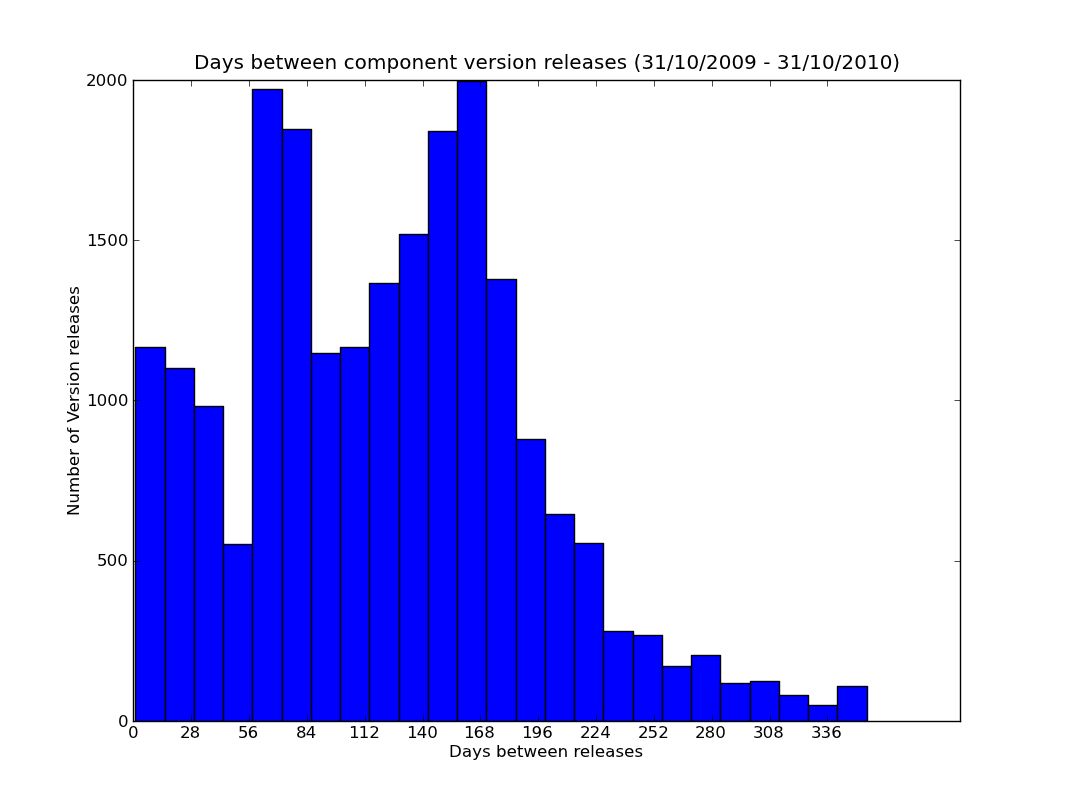
\includegraphics[width=\textwidth]{ubuntusimulationpics/versionreleasedistribution}
  \caption[labelInTOC]{Distribution of the releases of component versions between 31/10/2009 - 31/10/2010}
  \label{comeponentversionreleases}
\end{center}
\end{figure}

There are two points on this graph are noteworthy, firstly there is a large amount of components that release after 3 and 6 months.
Secondly there is a smaller but significant amount of components that have been released less than a month after the previous release.

The release of components after 3 or 6 month is probably due to the 6 monthly release cycle of Ubuntu.
Where individual components will release new versions for each Ubuntu release for it to be included.

\subsubsection{Effects of these releases}
%%%If this happens a lot, then these effects will happen
If this kind of release happens frequently to components in a repository, it causes much more change for a progressive user,
and standard strategies leave both conservative and progressive users vulnerable to the possible bug.

%%%A progressive user will experience a great deal more change with little benefit
The main effect of this kind of release causes to a progressive user is their system will go through more changes with little benefit.
As a progressive user will update frequently, it means they may upgrade to each release of a component.
As the time between the releases are so close to each other this only introduces more risk, and has little benefit for the system.

%%%Both types of users are vulnerable if the bug effects them
Another problem caused by this type of release is that if the bug effects the system, conservative users as well as progressive users are vulnerable.
Conservative users, although they update less frequently do update sometimes.
The time in which they update could be between one of these releases and then the bug can be introduced into their system, 
causing them to update once more, maybe introducing another bug.


\subsubsection{Criteria}   
The effects caused by these components that release soon after, i.e. within a month, of a previous release can be mitigated by taking into account when a component was released.
This criteria will then wait a certain amount of time once a package has been released, ensuring that no more releases are coming.
This idea is called ``Stable Version'', the main parameter that is required is the time in which to wait for a package to become stable.

This stable release criteria is defined as a hard constraint that can be added to a users update criteria.
%%%TODO This constraint is added, though it is not a criteira, TODO if there is only one package that has been released recently and asked to be installed will cause conflict

To test this criteria, to see if it reduces the effects of a set of user values is selected from the logs and extremes to build sets of user actions.
Through altering our progressive and conservative criteria to include the stable version criteria a range of values for the parameter of stable version is tested and measured for performance.
The criteria are altered to ``-stableversion(N),-removed,-new,-uptodatedistance'' and ``-stableversion(N),-uptodatedistance,-removed,-new'' where N is a number from a selected range.

\subsubsection{Results}
Compare against extreme and normal update distances.

\subsubsection{Conclusions}
The addition of the stable version criteria is shown to improve both the conservative and progressive user criteria.

It also shows that updating daily with a large stable version parameter is more conservative with better metrics than updating less frequently with no parameter.

\subsection{How do major releases effect component evolution?}
A release of a component system is a milestone in the system and repository.
It involves the cooperation of many parties, including the component systems managers, and the component developers.
This usually has many formal aspects to it, in Ubuntu there is an official schedule which is followed, an example shown in figure \ref{ubuntuSchedule}.

\begin{figure}[htp]
\begin{center}
  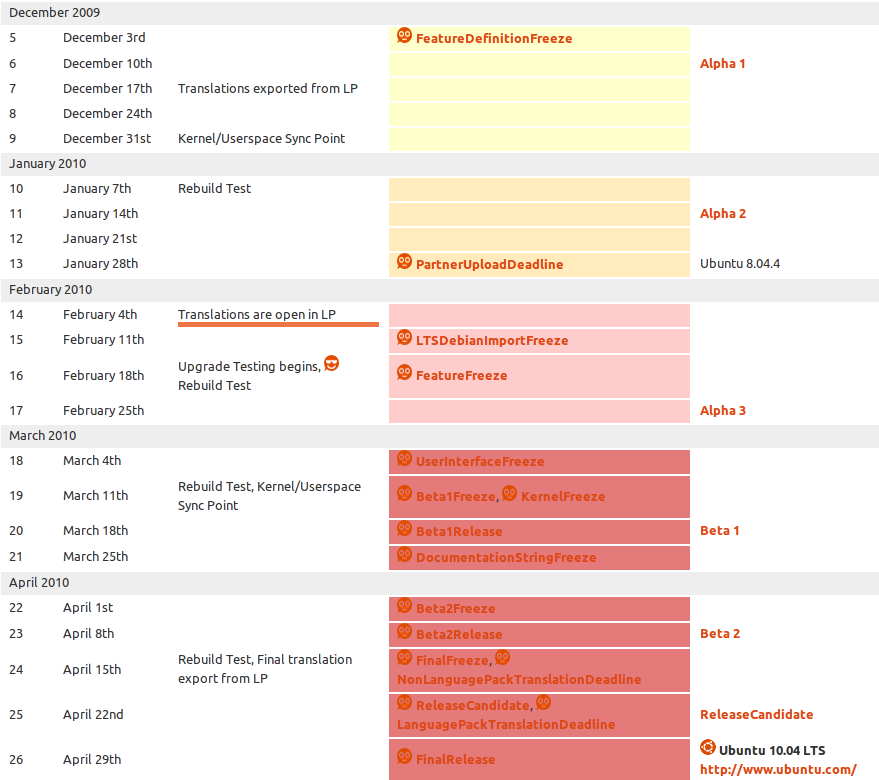
\includegraphics[width=\textwidth]{ubuntusimulationpics/ubunturelease}
  \caption[labelInTOC]{The Ubuntu release schedule from https://wiki.ubuntu.com/LucidReleaseSchedule accessed 6/3/2012}
  \label{ubuntuSchedule}
\end{center}
\end{figure}

This schedule involves multiple releases assuring quality of the final version, 
and freezes on different aspects of the components and system to assure that they do not change once the required quality has been found.


The consequences such schedules have on a repository is can be measured through comparing the activity of components added to the repository when compared to the different Ubuntu releases.
The amount of components added to the repository in relation to four different releases can be seen in figure \ref{ubuntureleases}.

\begin{figure}[htp]
\begin{center}
  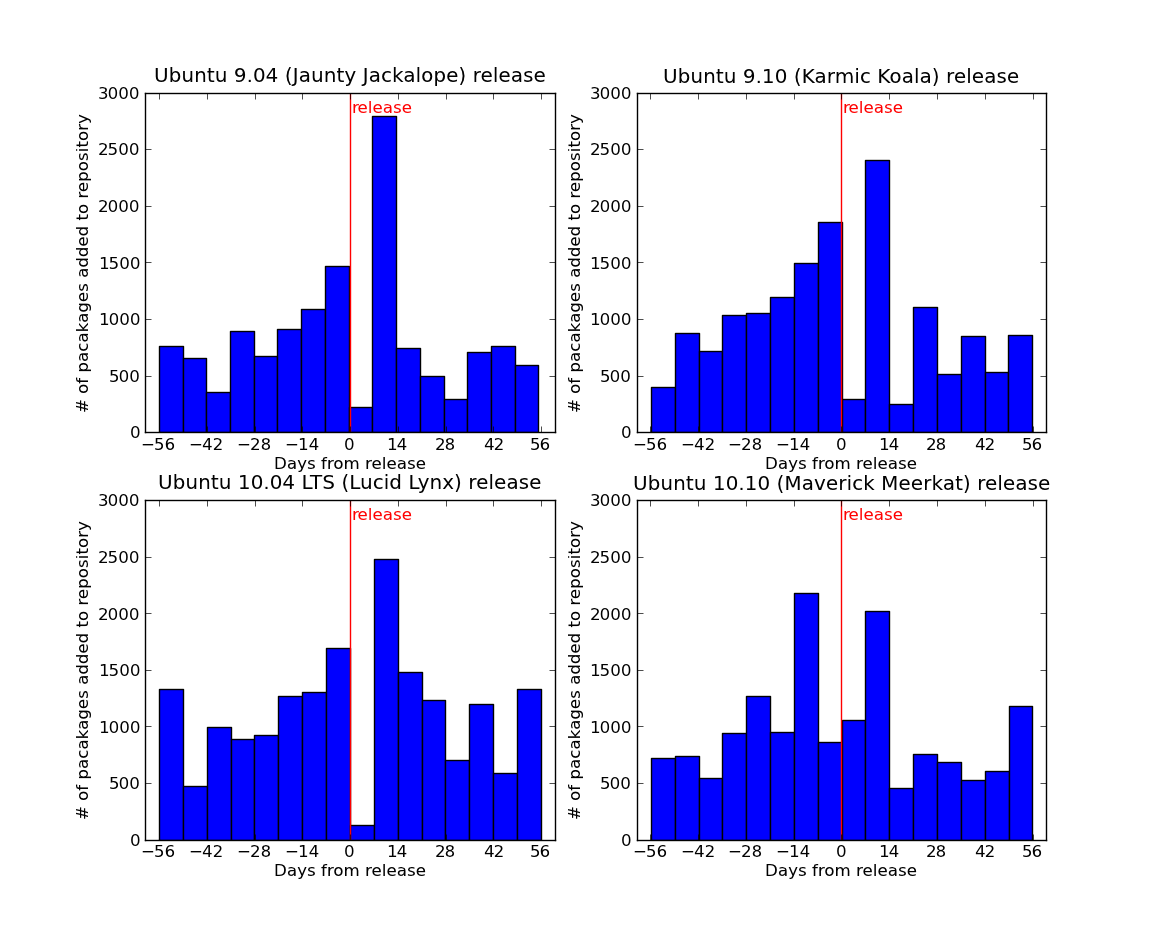
\includegraphics[width=\textwidth]{ubuntusimulationpics/releasedatepacakges}
  \caption[labelInTOC]{The amount of packages added to the repository in relation to the Ubuntu releases}
  \label{ubuntureleases}
\end{center}
\end{figure}

Three patterns can be seen in this figure, a build up to a release, a break after a release and a massive addition of components about two weeks after.

The build up to the release of components being added to the repository is probably component developers adding their latest versions to be included in the new major release.
The break after the release, where there is significantly less components added to the repository, is likely an effect of the freeze on addition of comopnents, while the new release stabilises.

The massive addition of components usually two weeks after the release, is the most concerning aspect.
Likely it is either a situation described previously where developers are receiving bug reports and adding fixes, 
or developers adding components that were unable to be added due to the freezes imposed on the repository. 

This leads to the question of how do these releases effect the evolution of a component system, because clearly they effect the repository.

\subsubsection{Experiment}
The simulations configuration is defined to execute over the Ubuntu 10.04 (Lucid Lynx) release.
Therefore, this is used to identify some of the effects that occur due to major releases in a repository.
There are some difference to reality that must be defined, firstly   

The previously defined experiments are now analysed with a closer eye on this period before and after a release, to analyse the effects on different criteria.
Specifically, the changes made to find if the changes increase in relation to the release date, and 

\subsubsection{Results}
The changes made to the system around the release date can be seen to increase significantly.

The changes made using the stable criteria, are delayed, but also less as it waits for the system to stabalise.

\subsubsection{Conclusion}
Major releases effect the evolution of a component systems.

This effect is felt mostly by users the update often and those that update progressivly.

The stable criteria as defined mitigates some of this effect of this system by waiting for the components to stabalize in their changes.

% \subsection{What is the effect of updating for while satisfying maximising recomends satisfaction?}
% As well as their explicit dependencies, components can define dependencies that they recommend should be installed.
% These components are usually what has been tested and are likely to interact with little friction with other components.
% Therefore, by satisfying these recomendation the system should be functional, though these recomendation may conflict with other users criteria.
% 
% Installing recommended pieces of software may duplicate functionality in  
% 
% Testing how the maximising the recomendations impacts the evolution of the system using the three 
% 
% Specifically, 10 runs for each of 5 selected users where executedusing the a
% conservative criteria ``-removed,-new,-unsat\_recommends,-uptodatedistance'', a progressive criteria ``-unsat\_recommends,-uptodatedistance,-removed,-new''
% and a mixed criteria ``-removed,-unsat\_recommends,-uptodatedistance,-new''.
% 
% \subsubsection{Results}
% Graphs of system size, system change are compared to the typical P2, APT and extreme progressive crtieria.
% 
% Life cycle, clearly the first update will hurt the most.
% 
% Show the trade offs.
% 
% 
% \subsubsection{Conclusion}
% Installing with recommendation may be prefered to increase stability, though it significantly increases the amount of change in a system, mostly at the begning.

\subsection{Graph metrics to lower change?}
The selection of the newest version is selected as it is presumed that the highest version is the best in the range of possible versions.
Graph metrics can measure the amount a component can be potentially be used.
However, given that the repository is always changing and newer versions are always added, the relationship between these metrics and their components,
is first needed to be studied in order to access this hypothesis.

%%%TODO
First we explore the way in which these values change over versions of components, because if it is linear it will not work.
If the value always increases over versions then the latest version will always be installed,
If the value always decreases then the least updated version is always installed, either of which can be much more easily calculated.

\subsubsection{Results}
Results from graph metrics that can be used.
Given a change, the number of components that depend on the changed components can be measured.
This could be described as the set of components that may through an error given a certain change.
If this is lower than using other conservative criteria this would be a sucessful use of criteira.

\subsection{What are the effects of a typical installation criteria?}
When a component is installed into a system the criteria is always conservative as the installation action is meant to change only parts of the system related to the selected components to install.
For instance, if the install criteria was progressive like ``-uptodatedistance,-removed,-new'', it would update the system when it installed, which is not its goal.

The extent at which the installation criteria is conservative can be altered per user.
The most conservative criteria criteria as described in \ref{strategies}  is ``-changed,-uptodatedistance'', this will only change a package if necessary and try to install uptodate versions.
The least conservative criteria that a user may want is ``-removedcomponent,-uptodatedistance,-changed'', this will first minimise removing any component from the original system,
then select uptodate components, finally minimising change.

Installation distributions can be measured in two different dimensions, how many components per install, and how often they select to install.
This gives us four typical users; a user who installs very few components infrequently; 
a user who installs very few components often;
a user who installs many components infrequently,
and a user who installs many components often install many components often.

Creating such user distributions is a difficult problem, as it involves creating realistic user interactions, which is very difficult.
Therefore, 4 user install distribution from user submitted logs who subjectively meet these descriptions have been selected to represent the extreme users.
These are simulated with the above defined criteria, to analyse the effect on component evolution.

Given the significant randomness that is involved with the installation property, 30 different user action sets have been generated for each user.

%TODO look at how the top 100 components install effect the system, for different criteria, how many components they add, and what common components are added!

\subsection{Results}
The effects of using these install criteria, focus on the 

How much change does a typical install cause (also investigated in \citep{Jenson2010})

\subsection{Conclusion}
This criteria is difficult to 

\subsection{Effects of installing and updating of typical users?}
Throughout these questions, criteria for updating and installtion, for progressive and conservative users have been defined and studied for their impacts on component system evolution.
It is asked here what impact these have overall, when combined together and simulated.

Specifically, four users will be created that express the sterotypes of extreme and moderarte versions of progressive and conservateive users.
Then 4 user install distributions and update probabilities will be selected from the user submitted logs that represent these user types and be simulated with 30 different user action sets each.

With these typical users, the simulation is run.
\subsubsection{Results}
The results are presented specifically showing the two main goals of limited uptodate

\section{Summary}
%%%A list of the answers gained from the questions
